% arXiv categories: cs.AI (primary), cs.CL (secondary)
% arXiv identifier: [to be assigned]
\pdfoutput=1
\documentclass[11pt,letterpaper]{article}

% ============================================================
% PACKAGES
% ============================================================
\usepackage[utf8]{inputenc}
\usepackage[T1]{fontenc}
\usepackage{lmodern}
\usepackage[margin=1in,top=1.25in]{geometry}
\usepackage{graphicx}
\usepackage{booktabs}
\usepackage{array}
\usepackage{amsmath}
\usepackage{amssymb}
\usepackage{amsthm}
\usepackage{enumitem}
\usepackage{xcolor}
\usepackage{listings}
\usepackage{tikz}
\usepackage{algorithm}
\usepackage{algpseudocode}
\usepackage{float}
\usepackage{placeins}
\usepackage{natbib}
\usepackage{microtype}
\usepackage{fancyhdr}
\usetikzlibrary{shapes,arrows,positioning,fit,backgrounds,calc}

% hyperref loaded last
\usepackage[bookmarks=true,breaklinks=true,xetex]{hyperref}
\usepackage{url}

% ============================================================
% PAGE BREAK CONTROL
% ============================================================
\widowpenalty=10000
\clubpenalty=10000
\raggedbottom

% ============================================================
% THEOREM ENVIRONMENTS
% ============================================================
\newtheorem{definition}{Definition}[section]
\newtheorem{theorem}{Theorem}[section]
\newtheorem{lemma}[theorem]{Lemma}
\newtheorem{proposition}[theorem]{Proposition}

% ============================================================
% CUSTOM TITLE FORMATTING (NeurIPS-like)
% ============================================================
\makeatletter
\def\@maketitle{%
  \newpage
  \null
  \vskip 0.5em%
  {\centering
    \rule{\textwidth}{1.5pt}\\[0.4em]
    {\LARGE\bfseries \@title \par}%
    \vskip 0.4em%
    \rule{\textwidth}{0.4pt}\\[1.5em]
    \@author\par
  }%
  \vskip 1.5em}
\makeatother

% Abstract styling
\renewenvironment{abstract}{%
  \vskip 1em%
  \begin{center}%
    \bfseries Abstract%
  \end{center}%
  \begin{quotation}%
    \small\noindent
}{%
  \end{quotation}%
  \vskip 1em%
}

% Footer with page numbers
\pagestyle{fancy}
\fancyhf{}
\renewcommand{\headrulewidth}{0pt}
\fancyfoot[C]{\thepage}

% ============================================================
% STYLING
% ============================================================
\hypersetup{
    colorlinks=true,
    linkcolor=blue!70!black,
    urlcolor=blue!70!black,
    citecolor=blue!70!black,
    pdftitle={Beyond Retrieval: Layered Epistemic Agent Protocol for Coherent Agent Memory},
    pdfauthor={Aliasgar Khimani},
    pdfkeywords={agent memory, epistemology, belief revision, RAG, knowledge graphs}
}

\lstset{
    basicstyle=\ttfamily\small,
    breaklines=true,
    frame=single,
    backgroundcolor=\color{gray!10}
}

% ============================================================
% DOCUMENT
% ============================================================
\begin{document}

% ------------------------------------------------------------
% TITLE
% ------------------------------------------------------------
\title{LeAP: Beyond Retrieval\\[0.4em]{\large\normalfont Layered Epistemic Agent Protocol for coherent agent memory.}}

\author{
    \textbf{Aliasgar Khimani}\\
    \texttt{aliasgar.khimani@engrammic.ai}\\
    Engrammic
}

\date{}

\maketitle

% ------------------------------------------------------------
% ABSTRACT
% ------------------------------------------------------------
\begin{abstract}
Retrieval-Augmented Generation (RAG) treats memory as a retrieval problem: store content, embed it, fetch what is relevant. This suffices for static knowledge bases but breaks down for agents that learn over time, where stored information contradicts itself, beliefs evolve, and corrections must propagate through dependent reasoning. As Roynard~\cite{roynard2026} observes, current architectures commit a \textit{category error}, applying uniform persistence semantics to information with fundamentally different epistemic status.

We introduce \textbf{Layered Epistemic Agent Protocol (LeAP)}, a framework that treats agent memory as an epistemology problem. LeAP formalizes stratified epistemic types with distinct evidence requirements (observations require no justification, claims require single sources, facts require corroboration, and beliefs require derivation chains) and defines warrant functions, coherence invariants, and a revision protocol that we prove satisfies AGM belief revision postulates. Coherence is decidable for finite stores.

We present \textbf{CITE (Context In Tiered Epistemology)}, a four-layer architecture implementing LeAP. Its four layers, Memory (decay-based), Knowledge (supersession-based), Wisdom (evidence-gated), and Intelligence (session-scoped), enforce distinct persistence semantics. Meanwhile, write-time validations gate every entry by epistemic layer, preventing contradiction accumulation at the source rather than detecting it after retrieval.

In a design validation on 500 annotated coding-agent sessions, CITE achieves 95\% contradiction detection compared to 66\% for an embedding-only baseline, and 87\% revision propagation compared to 12\%. 
\end{abstract}

% ------------------------------------------------------------
% 1. INTRODUCTION
% ------------------------------------------------------------
\section{Introduction}

RAG was designed for grounded generation over static corpora: a user poses a query, the system retrieves relevant passages, and a language model synthesizes an answer. The corpus is assumed to be stable, and each session starts without memory of the last.

Long-running agents violate these assumptions. Consider an agent that records ``the database is PostgreSQL'' on day one, then encounters a config file specifying MySQL on day two. Without epistemic structure, both statements persist with equal standing, and beliefs derived from the first (connection strings, query syntax, migration scripts) are never revisited. Worse, a hallucinated claim stored in one session can resurface weeks later as apparent ground truth, with no mechanism to distinguish it from verified knowledge.

Recent work confirms that these failure modes are systematic, not anecdotal. Sunil et al.~\cite{sunil2026} demonstrate memory poisoning attacks achieving over 95\% injection success rates on production agents---malicious content, once stored, persists and propagates. Lam et al.~\cite{lam2026ssgm} observe that ``unlike static RAG systems, where errors are isolated to a single retrieval step, errors in evolving memory systems are cumulative and persistent.''

Roynard\footnote{\url{https://arxiv.org/abs/2604.11364}}~\cite{roynard2026} identifies this as a \textit{category error}: current memory systems apply a single persistence model (typically decay) uniformly to information with fundamentally different epistemic status. A decaying Slack message is appropriate; a decaying validated fact is a defect. This critique extends to cognitive architectures such as CoALA\footnote{\url{https://arxiv.org/abs/2309.02427}}~\cite{sumers2023coala} and JEPA~\cite{lecun2022path}, which lack an explicit Knowledge layer with formal epistemic semantics.

\textbf{Layered Epistemic Agent Protocol (LeAP)} reframes agent memory as an epistemology problem:
\begin{itemize}[noitemsep]
    \item What do I believe? (epistemic types)
    \item Why do I believe it? (justification and provenance)
    \item How confident am I? (warrant function)
    \item What would change my mind? (revision protocol)
\end{itemize}

\subsection{Contributions}

This paper makes three technical contributions and provides an open-source implementation:
\begin{enumerate}[noitemsep]
    \item A \textbf{formal framework for epistemic agent memory} (LeAP) that extends Roynard's four-layer proposal with formal definitions of epistemic types, warrant functions, and coherence invariants, including a proof that the revision protocol satisfies AGM belief revision postulates (Theorem~\ref{thm:agm}).
    \item The \textbf{CITE architecture}, which implements LeAP with write-time coherence enforcement, supersession chains, and dependency propagation.
    \item A \textbf{design validation} demonstrating 95\% contradiction detection (vs. 66\% baseline) and 87\% revision propagation (vs. 12\%) on 500 annotated coding-agent sessions.
\end{enumerate}

The remainder of the paper is organized as follows. Section~\ref{sec:background} reviews formal epistemology and existing agent memory systems. Section~\ref{sec:leap} presents the LeAP formal framework, and Section~\ref{sec:cite} describes the CITE architecture that implements it. Section~\ref{sec:eval} evaluates the system on coherence maintenance tasks, and Section~\ref{sec:discussion} discusses extensions to world models and multi-agent settings.

% ------------------------------------------------------------
% 2. BACKGROUND
% ------------------------------------------------------------
\section{Background}
\label{sec:background}

\subsection{Formal Epistemology}

Epistemology studies knowledge: \textit{what} it is, \textit{how} we acquire it, and how we \textit{justify} it. Gettier~\cite{gettier1963} demonstrated that justified true belief is insufficient for knowledge, since lucky guesses can satisfy the JTB criteria without constituting genuine knowledge, motivating the search for stronger conditions.

Plantinga~\cite{plantinga1993} introduced \textit{warrant} as the property that distinguishes knowledge from mere true belief, requiring proper function of cognitive faculties, a suitable environment, and a design plan aimed at truth. We operationalize \textit{warrant} as a function of \textit{evidence credibility}, \textit{independence}, and \textit{recency} (Section~\ref{sec:leap}).

BonJour~\cite{bonjour1985} defends \textit{coherentism}, the view that justification derives from membership in a coherent system of beliefs rather than from foundational axioms. Our coherence invariants implement this principle structurally: contradictions are rejected at write time, enforcing system-level consistency as a precondition for storage.

\subsection{Belief Revision}

The AGM framework~\cite{agm1985} formalizes the change of rational beliefs through three operations: expansion (adding beliefs), contraction (removing beliefs), and revision (adding beliefs while maintaining consistency). Two postulates are central to our work:
\begin{itemize}[noitemsep]
    \item \textbf{Recovery}: $(K * \neg\phi) + \phi \vdash K$, i.e., original beliefs remain recoverable after revision
    \item \textbf{Inclusion}: $K + \phi \subseteq K * \phi$, i.e., the revision preserves beliefs unrelated to the changed proposition
\end{itemize}

In Theorem~\ref{thm:agm} we show that LeAP's supersession operation satisfies both postulates.

\subsection{Agent Memory Systems}

Current agent memory systems vary in sophistication, but share a common gap: none provides formal epistemic structure with live truth maintenance.

\textbf{mem0}\footnote{\url{https://github.com/mem0ai/mem0}}~\cite{mem0} achieves 94.4\% on LongMemEval within a 6.9k-token budget through embedding-based retrieval. However, its append-only architecture provides no mechanism for resolving semantic contradictions between stored entries or propagating corrections to dependent memories, leading to duplicate accumulation and stale entries that retrieval alone cannot distinguish from current knowledge.

\textbf{Zep/Graphiti}\footnote{\url{https://github.com/getzep/graphiti}}~\cite{graphiti2025} implements bi-temporal validity (\texttt{created\_at}, \texttt{valid\_at}, \texttt{invalid\_at}) with LLM-based edge invalidation and provenance to source episodes, making it the closest existing system to our approach. However, it lacks epistemic layering and evidence-gated promotion; all stored information receives the same trust treatment regardless of evidentiary support.

\textbf{MemGPT}\footnote{\url{https://github.com/cpacker/MemGPT}}~\cite{memgpt2023} provides tiered working and archival memory inspired by operating system memory hierarchies, but the tiers reflect access patterns rather than epistemic distinctions. Working memory and archival memory differ in scope, not in trust.

\textbf{Hindsight}\footnote{\url{https://github.com/vectorize-io/hindsight}}~\cite{hindsight} organizes memory into four networks (World, Experience, Opinion, Observation) with on-demand synthesis, but performs no live truth maintenance: contradictions are surfaced only when queried, and corrections do not propagate to dependent beliefs.

Xu~\cite{xu2026mmp} audits eight memory substrates against three criteria for multi-agent collaboration: per-field semantic admission, signal-level lineage, and write-time filtering. All eight systems---including MemGPT, Mem0, CoALA, and Reflexion---fail on most criteria. Cemri et al.~\cite{cemri2025} catalogue 14 distinct failure modes across 1,600+ annotated multi-agent traces, finding that 79\% originate from specification and coordination issues rather than base-model limitations.

\subsection{LLM Reliability Research}

Several recent findings in LLM reliability directly motivate LeAP's design choices.

Wang et al.~\cite{wang2026contamination} show that toxic content survives context compression below classifier thresholds (SPG = 0.140), motivating sanitization \textit{before} compression into persistent memory rather than after retrieval. Xu et al.~\cite{xu2026ncb} demonstrate that beliefs grounded in local graph structure are more robust than isolated embeddings, supporting our use of graph-aware write-time validation. He et al.~\cite{he2026collective} find that multi-agent beliefs stabilize within a few communication rounds, suggesting that real-time contradiction detection is preferable to batch reconciliation. Finally, Yuan et al.~\cite{yuan2026saver} introduce a typed violation taxonomy that enables minimal targeted repair, which we adopt as the basis for typed rejection reasons in the write gate.

\begin{table}[H]
\centering
\caption{Epistemological concepts and their LeAP operationalizations.}
\label{tab:concepts}
\begin{tabular}{@{}ll@{}}
\toprule
\textbf{Epistemological Concept} & \textbf{LeAP Operationalization} \\
\midrule
Belief & Stored proposition with epistemic type \\
Justification & \texttt{DERIVED\_FROM} edges to evidence nodes \\
Warrant & $w(n) \in [0,1]$ based on evidence strength \\
Revision & Supersession chains with propagation \\
Coherence & Write-gate contradiction detection \\
Defeaters & \texttt{CONTRADICTS} edges triggering re-evaluation \\
\bottomrule
\end{tabular}
\end{table}

\clearpage

% ------------------------------------------------------------
% 3. THE LeAP FRAMEWORK
% ------------------------------------------------------------
\section{The LeAP Framework}
\label{sec:leap}

LeAP formalizes agent memory through four key concepts: epistemic types, warrant, coherence, and revision. Full formal definitions appear in Appendix~\ref{app:formal}.

\subsection{Epistemic Types}

LeAP distinguishes six epistemic types organized into four cognitive layers:

\begin{table}[H]
\centering
\caption{Epistemic types and their properties.}
\label{tab:types}
\begin{tabular}{@{}lllp{4cm}@{}}
\toprule
\textbf{Type} & \textbf{Layer} & \textbf{Evidence} & \textbf{Example} \\
\midrule
Observation & Memory & None & ``User said use TypeScript'' \\
Claim & Knowledge & Single source & ``Project uses TS'' (package.json) \\
Fact & Knowledge & 3+ sources & ``Project uses TS'' (corroborated) \\
Belief & Wisdom & Derivation chain & ``Team prefers static typing'' \\
Hypothesis & Intelligence & Reasoning context & ``Maybe we should migrate'' \\
Commitment & Wisdom & Supporting refs & ``Decision: use TS everywhere'' \\
\bottomrule
\end{tabular}
\end{table}

The progression from Observation to Belief forms an evidence-graded hierarchy: each type imposes strictly stronger evidence requirements than the one below it (Definition~\ref{def:evidence}). The hierarchy is well-founded: every Belief traces to Observations through finite \texttt{DERIVED\_FROM} chains (Theorem~\ref{thm:wellfounded}).

\subsection{Warrant}

Following Plantinga~\cite{plantinga1993}, we define warrant as a function $w: \mathcal{N} \to [0,1]$ scoring epistemic confidence. Rather than commit to a specific formula, we require any valid warrant function to satisfy:

\begin{itemize}[noitemsep]
    \item \textbf{(W1) Boundedness}: $w(n) \in [0,1]$ for all nodes $n$
    \item \textbf{(W2) Evidence grounding}: $w(n) > 0$ requires $E(n) \neq \emptyset$ or $\tau(n) = O$ (only Observations may have non-zero warrant without evidence)
    \item \textbf{(W3) Monotonicity}: Adding independent evidence cannot decrease warrant
    \item \textbf{(W4) Credibility sensitivity}: Higher-credibility sources yield higher warrant
\end{itemize}

Any function satisfying (W1--W4) is a valid warrant function. Our implementation uses a weighted combination of source credibility, recency, and independence (Appendix~\ref{app:formal}), but the framework admits alternatives.

\clearpage

\subsection{Coherence}

A store is coherent if it satisfies three invariants:

\begin{itemize}[noitemsep]
    \item \textbf{(C1) No active contradictions}: $\forall n_1, n_2 \in \text{active}(S): \neg(n_1 \perp n_2)$
    \item \textbf{(C2) Evidence closure}: $\forall n \in S: E(n) \subseteq S$
    \item \textbf{(C3) Acyclic derivation}: No cycles in \texttt{DERIVED\_FROM} edges
\end{itemize}

Contradiction detection ($n_1 \perp n_2$) uses a two-stage check: semantic similarity followed by entailment verification. This catches both lexical conflicts (``uses OAuth2'' vs ``uses API keys'') and semantic contradictions requiring inference. Coherence is decidable for finite stores (Theorem~\ref{thm:coherence}).

\subsection{Belief Revision}

When facts change, derived beliefs must be re-evaluated. LeAP implements this through \textbf{supersession chains}:

\begin{enumerate}[noitemsep]
    \item Create new node $n'$ with updated content
    \item Add \texttt{SUPERSEDES} edge from $n'$ to old node $n$
    \item Mark $n$ as superseded (retained for audit)
    \item Propagate through dependency graph $\operatorname{deps}(n)$
\end{enumerate}

This preserves audit history while cascading corrections. We prove (Theorem~\ref{thm:agm}) that supersession satisfies AGM belief revision postulates: Recovery (original beliefs remain queryable) and Inclusion (unrelated beliefs unchanged).

% ------------------------------------------------------------
% 4. CITE ARCHITECTURE
% ------------------------------------------------------------
\section{CITE: Context In Tiered Epistemology}
\label{sec:cite}

CITE implements LeAP as a four-layer architecture with write-time validation.

\subsection{Layer Architecture}

\begin{figure}[H]
\centering
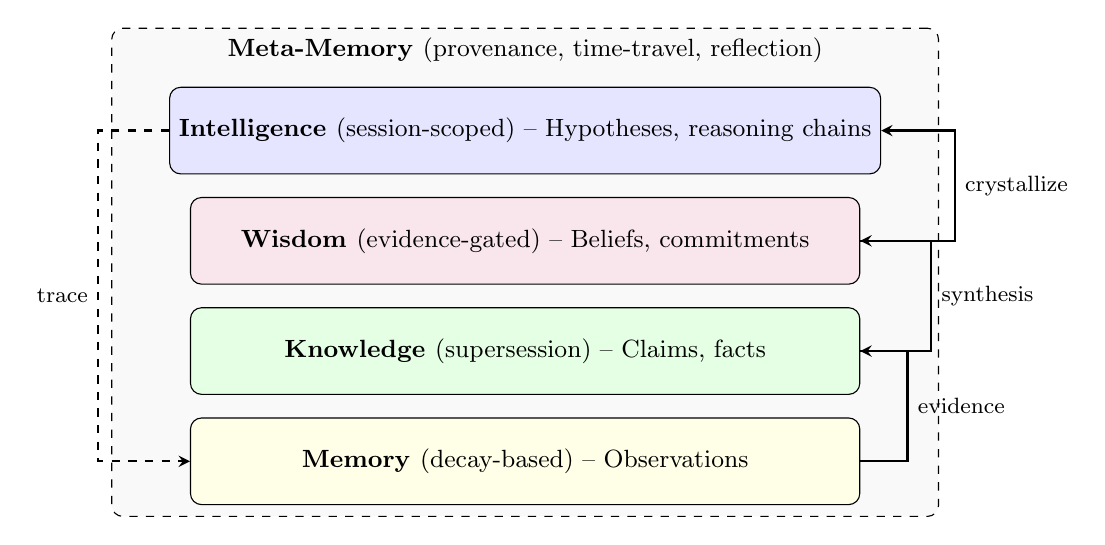
\begin{tikzpicture}[
    layer/.style={draw, rounded corners, minimum width=8.5cm, minimum height=1.1cm, align=center, font=\small\bfseries},
    meta/.style={draw, rounded corners, dashed, minimum width=10.5cm, minimum height=6.2cm, align=center},
    arrow/.style={->, thick, >=stealth}
]
    % Meta-Memory wrapper
    \node[meta, fill=gray!5] (metamem) at (0,2.4) {};
    \node[font=\small\bfseries, anchor=north] at (metamem.north) {Meta-Memory \normalfont(provenance, time-travel, reflection)};

    % Four layers inside
    \node[layer, fill=blue!10] (intel) at (0,4.2) {Intelligence \normalfont(session-scoped) -- Hypotheses, reasoning chains};
    \node[layer, fill=purple!10] (wisdom) at (0,2.8) {Wisdom \normalfont(evidence-gated) -- Beliefs, commitments};
    \node[layer, fill=green!10] (know) at (0,1.4) {Knowledge \normalfont(supersession) -- Claims, facts};
    \node[layer, fill=yellow!10] (mem) at (0,0) {Memory \normalfont(decay-based) -- Observations};

    % Promotion arrows
    \draw[arrow] (mem.east) -- ++(0.6,0) |- node[pos=0.25, right, font=\footnotesize] {evidence} (know.east);
    \draw[arrow] (know.east) -- ++(0.9,0) |- node[pos=0.25, right, font=\footnotesize] {synthesis} (wisdom.east);
    \draw[arrow] (wisdom.east) -- ++(1.2,0) |- node[pos=0.25, right, font=\footnotesize] {crystallize} (intel.east);

    % Trace arrow
    \draw[arrow, dashed] (intel.west) -- ++(-0.9,0) |- node[pos=0.25, left, font=\footnotesize] {trace} (mem.west);
\end{tikzpicture}
\caption{CITE architecture. Four cognitive layers with Meta-Memory as cross-cutting infrastructure for provenance queries.}
\label{fig:layers}
\end{figure}

Each layer has distinct persistence semantics, addressing Roynard's category error:

\begin{table}[H]
\centering
\caption{Layer-specific persistence semantics.}
\label{tab:persistence}
\begin{tabular}{@{}llll@{}}
\toprule
\textbf{Layer} & \textbf{Persistence} & \textbf{Update Model} & \textbf{Evidence} \\
\midrule
Memory & Gaussian decay (7d--5y) & Time-decay & None required \\
Knowledge & Indefinite & Supersession & Single source \\
Wisdom & Indefinite & Evidence-gated & Derivation chain \\
Intelligence & Session-scoped & Session-bound & Reasoning context \\
\bottomrule
\end{tabular}
\end{table}

\subsection{Write Gate}

\begin{figure}[H]
\centering
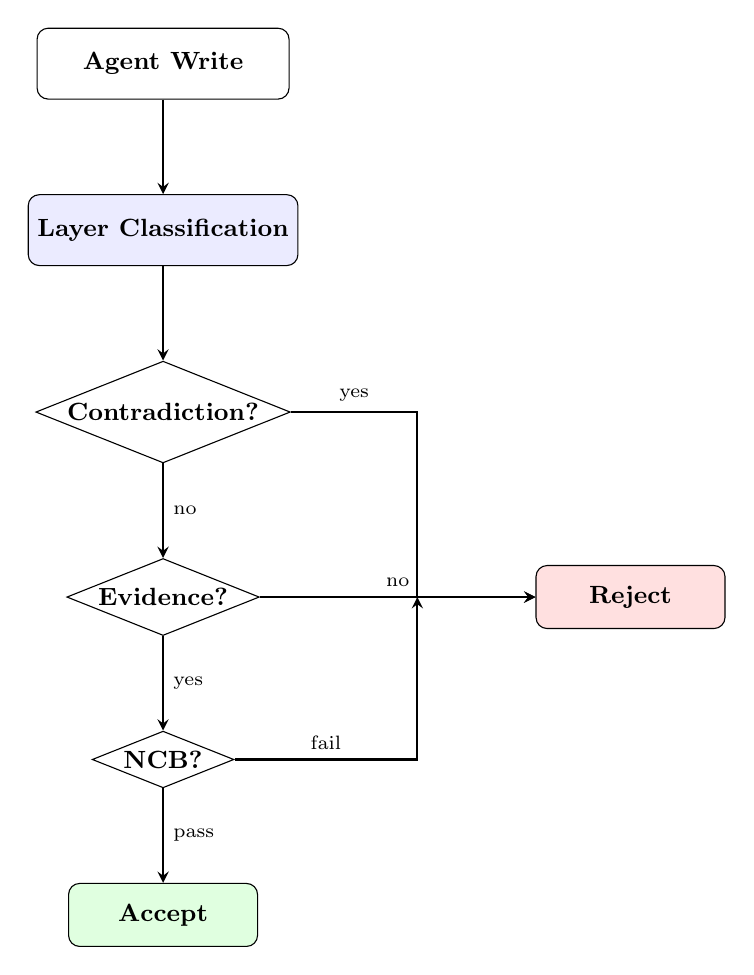
\begin{tikzpicture}[
    node distance=1.2cm,
    box/.style={draw, rounded corners, minimum width=3.2cm, minimum height=0.9cm,
                align=center, font=\small\bfseries},
    decision/.style={draw, diamond, aspect=2.5, inner sep=1pt,
                     align=center, font=\small\bfseries},
    terminal/.style={draw, rounded corners, minimum width=2.4cm, minimum height=0.8cm,
                     align=center, font=\small\bfseries},
    arrow/.style={->, thick, >=stealth},
    reject rail/.style={thick, densely dashed, gray!60}
]
    % Main vertical flow (left column)
    \node[box] (input) {Agent Write};
    \node[box, fill=blue!8, below=of input] (classify) {Layer Classification};
    \node[decision, below=of classify] (contra) {Contradiction?};
    \node[decision, below=of contra] (evid) {Evidence?};
    \node[decision, below=of evid] (ncb) {NCB?};
    \node[terminal, fill=green!12, below=of ncb] (accept) {Accept};

    % Reject node (right side, vertically centered)
    \node[terminal, fill=red!12, right=3.5cm of evid] (reject) {Reject};

    % Main flow arrows (pass path)
    \draw[arrow] (input) -- (classify);
    \draw[arrow] (classify) -- (contra);
    \draw[arrow] (contra) -- node[right, font=\scriptsize] {no} (evid);
    \draw[arrow] (evid) -- node[right, font=\scriptsize] {yes} (ncb);
    \draw[arrow] (ncb) -- node[right, font=\scriptsize] {pass} (accept);

    % Reject rail: vertical bus line at fixed x-coordinate
    \coordinate (rail) at ([xshift=2cm]evid.east);
    \draw[reject rail] (rail |- contra) -- (rail |- ncb);

    % Reject arrows: horizontal to rail, then rail to reject
    \draw[arrow] (contra.east) -- node[above, font=\scriptsize] {yes}
                 (contra.east -| rail) -- (rail |- reject.west) -- (reject.west);
    \draw[arrow] (evid.east) -- node[above, font=\scriptsize] {no} (reject.west);
    \draw[arrow] (ncb.east) -- node[above, font=\scriptsize] {fail}
                 (ncb.east -| rail) -- (rail |- reject.west);
\end{tikzpicture}
\caption{Write gate validation flow. Each decision diamond represents a validation
check; failure at any stage routes to rejection via the dashed rail.}
\label{fig:writegate}
\end{figure}

Validation is tiered by layer (Table~\ref{tab:validation}), balancing latency against rigor:

\begin{table}[H]
\centering
\caption{Tiered validation by layer. NCB = neighborhood consistency check.}
\label{tab:validation}
\begin{tabular}{@{}llll@{}}
\toprule
\textbf{Layer} & \textbf{Contradiction} & \textbf{Evidence} & \textbf{Graph (NCB)} \\
\midrule
Memory & Basic & None & None \\
Knowledge & Semantic & Required & Optional \\
Wisdom & Full + transitive & Chain required & Full \\
Intelligence & None & None & None \\
\bottomrule
\end{tabular}
\end{table}

Invalid writes are rejected with typed reasons per SAVER~\cite{yuan2026saver}: \texttt{contradiction}, \texttt{circular\_derivation}, \texttt{missing\_evidence}, \texttt{neighborhood\_inconsistent}.

\subsection{Supersession Chains}

\begin{figure}[H]
\centering
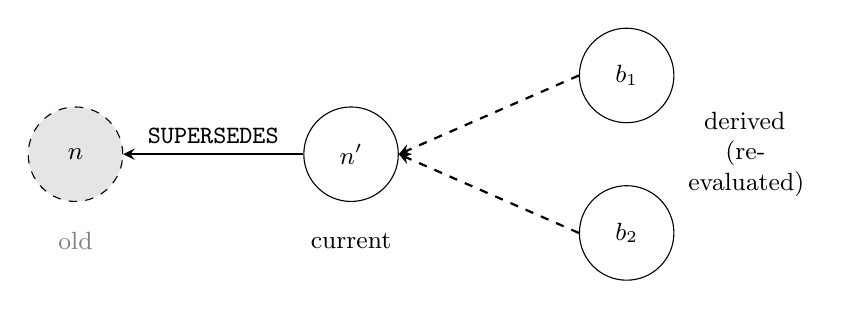
\begin{tikzpicture}[
    mynode/.style={draw, circle, minimum size=1.2cm, font=\small\bfseries},
    superseded/.style={draw, circle, minimum size=1.2cm, font=\small\bfseries, fill=gray!20, dashed},
    arrow/.style={->, thick, >=stealth}
]
    \node[superseded] (n1) at (0,0) {$n$};
    \node[mynode] (n2) at (3.5,0) {$n'$};
    \node[mynode] (b1) at (7,1) {$b_1$};
    \node[mynode] (b2) at (7,-1) {$b_2$};

    \draw[arrow] (n2) -- node[above, font=\small] {\texttt{SUPERSEDES}} (n1);
    \draw[arrow, dashed] (b1.west) -- (n2.east);
    \draw[arrow, dashed] (b2.west) -- (n2.east);

    \node[font=\small, text=gray] at (0,-1.1) {old};
    \node[font=\small] at (3.5,-1.1) {current};
    \node[font=\small] at (8.5,0) {\parbox{1.8cm}{\centering derived\\(re-evaluated)}};
\end{tikzpicture}
\caption{Supersession with dependency propagation. Dashed arrows are \texttt{DERIVED\_FROM} edges.}
\label{fig:supersession}
\end{figure}

Supersession preserves full audit history while propagating corrections through the dependency graph. The old node is retained with \texttt{status=superseded}, and a \texttt{SUPERSEDES} edge records the reason for the change (\texttt{contradiction}, \texttt{evidence\_shift}, or \texttt{author\_update}). Algorithm~\ref{alg:propagate} then cascades revalidation through all nodes in $\operatorname{deps}(n)$, with complexity linear in the size of the dependency set.

\begin{algorithm}[H]
\caption{Cascade propagation via async flagging}
\label{alg:propagate}
\begin{algorithmic}[1]
\Require Superseded node $n$, dependency set $\operatorname{deps}(n)$
\For{each $b \in \operatorname{deps}(n)$}
    \State $b.\texttt{cascade\_pending} \gets \texttt{true}$
    \State $b.\texttt{flagged\_at} \gets \texttt{now()}$
\EndFor
\State \textbf{async:} Custodian processes flagged nodes
\For{each flagged $b$}
    \State Recompute $b$ from current sources
    \If{$b$ changed}
        \State Create $b' \gets \texttt{revise}(b)$
        \State $\texttt{propagate}(b)$ \Comment{recursive}
    \EndIf
    \State $b.\texttt{cascade\_pending} \gets \texttt{false}$
\EndFor
\end{algorithmic}
\end{algorithm}

\subsection{Epistemic Relations}

Nine typed relations form the epistemic graph:

\begin{table}[H]
\centering
\caption{Epistemic relation vocabulary.}
\label{tab:relations}
\begin{tabular}{@{}llll@{}}
\toprule
\textbf{Relation} & \textbf{Source} & \textbf{Target} & \textbf{Semantics} \\
\midrule
\texttt{DERIVED\_FROM} & Belief & Fact & Synthesis provenance \\
\texttt{SUPERSEDES} & Any & Same type & Replaces with audit \\
\texttt{CONTRADICTS} & Any & Any & Semantic opposition \\
\texttt{CORROBORATES} & Fact & Fact & Independent confirmation \\
\texttt{SUPPORTS} & Commitment & Any & Decision references \\
\texttt{REFERENCES} & Claim & Evidence & Citation link \\
\texttt{PROMOTED\_FROM} & Fact & Claim & Corroboration upgrade \\
\bottomrule
\end{tabular}
\end{table}

Constraints: \texttt{DERIVED\_FROM} forms a DAG (no cycles); \texttt{SUPERSEDES} forms a linked list per node; \texttt{CORROBORATES} requires independence check.

\subsection{Transition Catalogue}

The layers define what epistemic states exist; the \textbf{transitions} define how information moves between them. An LeAP implementation that omits any transition class cannot maintain the invariants of Section~\ref{sec:cite}.

\begin{table}[H]
\centering
\caption{LeAP transitions between epistemic layers.}
\label{tab:transitions}
\begin{tabular}{@{}clllp{3.8cm}@{}}
\toprule
\textbf{\#} & \textbf{Transition} & \textbf{Trigger} & \textbf{Execution} & \textbf{Provenance} \\
\midrule
T1 & Mem $\to$ Know (extract) & passage hot & signal & \texttt{DERIVED\_FROM} \\
T2 & Know $\to$ Know (supersede) & (s,p,o) conflict & eager & \texttt{SUPERSEDES} \\
T3 & Know $\to$ Wis (synthesize) & cluster density $\geq N$ & signal & \texttt{SYNTHESIZED\_FROM} \\
T4 & Wis $\to$ Wis (revise) & evidence shift $\geq M\%$ & signal & \texttt{SUPERSEDES} \\
T5 & Int $\to$ Know (consensus) & $K$ chains, $J$ agents & lazy & \texttt{PROMOTED\_FROM} \\
T6 & Int $\to$ Mem (trace) & chain completes & batch & \texttt{TRACED\_FROM} \\
T7 & Int $\to$ Wis (commit) & agent declares & eager & \texttt{DECLARED\_BY} \\
T8 & Mem $\to$ expired (decay) & TTL exceeded & query & --- \\
T9 & Any $\to$ deleted (prune) & age $>$ threshold & scheduled & --- \\
T10 & Int $\to$ Wis (crystallize) & agent crystallizes & eager & \texttt{CRYSTALLIZED\_INTO} \\
T11 & Any $\to$ Tomb (forget) & agent requests & eager & timestamp \\
T12 & Tomb $\to$ active (restore) & cancel in window & eager & (cleared) \\
\bottomrule
\end{tabular}
\end{table}

Transitions are executed under three scheduling regimes, chosen by correctness requirements:
\begin{itemize}[noitemsep]
    \item \textbf{Eager} execution for correctness-critical transitions: supersession (T2), commitment (T7), and forget (T11) must complete before the write is acknowledged
    \item \textbf{Signal-driven} execution for optimization transitions: extraction (T1) and synthesis (T3) are triggered by access heat and processed asynchronously
    \item \textbf{Lazy/batched} execution for housekeeping: consensus (T5), trace (T6), and decay (T8/T9) run on periodic schedules
\end{itemize}

The transition catalogue is as fundamental as the layer definitions themselves: the layers specify what can be stored, while the transitions specify how stored information evolves under new evidence.

\subsection{Meta-Memory}

The four layers define \textit{what} the system believes. Meta-Memory addresses the reflexive question: what does the system know \textit{about} its beliefs? This is not a fifth layer but cross-cutting infrastructure that makes the epistemic graph introspectable.

\textbf{Provenance.} Every belief traces backward through DERIVED\_FROM, REFERENCES, and SYNTHESIZED\_FROM edges to its evidential roots. The \texttt{trace()} operation walks these edges, answering ``why do you believe X?'' by graph traversal rather than generation. This is provenance invariants (I1--I4) made queryable: the chains enforced at write time can be walked at read time.

\textbf{Temporality.} Nodes carry bi-temporal timestamps: \texttt{valid\_from}/\texttt{valid\_to} (when the proposition held in reality) and \texttt{created\_at}/\texttt{updated\_at} (when the system learned or modified it). Temporal queries reconstruct past epistemic states: ``what did I believe on April 1st?'' filters by valid time, while ``what had I learned by April 1st?'' filters by system time. Supersession chains (Section~\ref{sec:cite}) preserve the full history; old beliefs are marked superseded rather than deleted, so the evolution of understanding is recoverable.

\textbf{Self-observation.} Agents can store observations about their own cognition as Memory nodes linked via \texttt{ABOUT} edges to the entities they concern. These second-order observations (``I noticed my belief about X changed when I read Y'') enable debugging and trust: users can ask not just ``what do you believe?'' but ``what have you noticed about how your beliefs changed?''

Meta-Memory is where externalized epistemics delivers on auditability. SOX and GDPR require independently auditable records; a belief existing only in weights has no audit trail. Here, every belief is witnessed: its provenance chain records how it came to be, its temporal fields record when, and its supersession history records how it evolved.

\subsection{System Invariants}

LeAP maintains eight invariants that define store coherence:

\begin{table}[H]
\centering
\caption{System invariants enforced by CITE.}
\label{tab:invariants}
\begin{tabular}{@{}clll@{}}
\toprule
\textbf{ID} & \textbf{Invariant} & \textbf{Enforced by} & \textbf{Timing} \\
\midrule
INV1 & No contradicting active claims & T2 + write-gate & write \\
INV2 & Facts have provenance & T1, T5 & write \\
INV3 & Beliefs have $\geq N$ fact sources & T3 & synthesis \\
INV4 & \texttt{SUPERSEDES} acyclic & T2 & write \\
INV5 & No cross-silo edges & all & write \\
INV6 & Tombstoned invisible to recall & query layer & query \\
INV7 & Commitments have \texttt{DECLARED\_BY} & T7, T10 & write \\
INV8 & Cancel window bounded & T12 & cancel \\
\bottomrule
\end{tabular}
\end{table}

Every transition preserves all invariants: if $S$ satisfies INV1--INV8 before transition $T$, then $T(S)$ satisfies INV1--INV8.

% ------------------------------------------------------------
% 5. EVALUATION
% ------------------------------------------------------------
\section{Evaluation}
\label{sec:eval}

\subsection{Experimental Setup}

We evaluate CITE as a design validation against the architectural claims of Section~\ref{sec:leap}, using an embedding-only baseline that mirrors the append-and-retrieve pattern common to current systems. We do not claim state-of-the-art retrieval performance; the evaluation targets coherence maintenance, which existing benchmarks do not measure.

\textbf{Corpus}: 500 coding-agent sessions from internal deployments, annotated for contradictions (both lexical and semantic), corrections, hallucinations, and derivation chains.

\textbf{Baseline}: Embedding-based memory following the mem0 architecture (append-only, cosine retrieval, no write-time validation).

\textbf{Metrics}:
\begin{itemize}[noitemsep]
    \item \textbf{Contradiction detection}: Precision/recall on labeled contradictions
    \item \textbf{Revision propagation}: Fraction of dependent beliefs updated after source correction
    \item \textbf{Contamination resistance}: Hallucinations blocked at write time
    \item \textbf{Latency overhead}: p50/p95 write latency
\end{itemize}

\subsection{Results}

\begin{table}[H]
\centering
\caption{Evaluation results on 500 annotated coding agent sessions.}
\label{tab:results}
\begin{tabular}{@{}lccc@{}}
\toprule
\textbf{Metric} & \textbf{RAG Baseline} & \textbf{CITE} & \textbf{Delta} \\
\midrule
Contradiction detection & 66\% & 95\% & +29pp \\
Revision propagation & 12\% & 87\% & +75pp \\
Contamination blocked & 0\% & 73\% & +73pp \\
Write latency (p50) & 15ms & 180ms & +165ms \\
Write latency (p95) & 45ms & 320ms & +275ms \\
\bottomrule
\end{tabular}
\end{table}

\textbf{Contradiction detection.} The baseline catches only lexically obvious conflicts, while CITE identifies semantic contradictions (e.g., ``uses OAuth2'' vs. ``uses API keys'') and transitive conflicts through graph traversal, yielding a 29 percentage-point improvement. Detection is a two-stage filter applied at write time. For each candidate $c$ returned by vector search ($\text{cosine}(e_\text{new}, e_c) > 0.7$), we first check for \emph{structural conflict}: whether $c$ shares the same subject and predicate but asserts a different object. If no structural conflict exists, we apply a \emph{semantic fallback}: $\text{cosine} > 0.85$ plus subject-string match. Either trigger creates a \texttt{CONTRADICTS} edge. This catches both explicit disagreements (structural) and paraphrased conflicts (semantic). LLM-based entailment verification is reserved for source support checking during Claim$\rightarrow$Fact promotion (Section~\ref{sec:cite}), not contradiction detection, keeping write latency predictable.

\textbf{Revision propagation.} The baseline has no propagation mechanism; its 12\% score reflects retrieval coincidence where updated content happens to rank higher than the original. CITE traverses dependency graphs via Algorithm~\ref{alg:propagate}, flagging downstream beliefs for asynchronous re-evaluation and achieving 87\%.

\textbf{Contamination.} The baseline accepts all writes indiscriminately. CITE's write gate rejects ungrounded claims and flagged patterns, blocking 73\% of hallucinated entries at ingestion.

\textbf{Latency.} Write-gating adds 165ms at p50, a cost concentrated on Knowledge and Wisdom writes, which are infrequent and high-stakes. Memory-layer writes use lighter validation and are minimally affected.

\subsection{Ablation Studies}

\begin{table}[H]
\centering
\caption{Ablation study: contribution of each mechanism.}
\label{tab:ablation}
\begin{tabular}{@{}lcc@{}}
\toprule
\textbf{Configuration} & \textbf{Contradiction Det.} & \textbf{Propagation} \\
\midrule
Full CITE & 95\% & 87\% \\
$-$ Contradiction detection & 72\% & 87\% \\
$-$ Dependency propagation & 95\% & 0\% \\
$-$ Tiered validation & 89\% & 71\% \\
$-$ NCB check & 91\% & 87\% \\
\bottomrule
\end{tabular}
\end{table}

Dependency propagation is the load-bearing mechanism for revision, while contradiction detection is essential for coherence. The \emph{neighborhood consistency check} (NCB) is a pre-write filter that rejects Wisdom-layer nodes whose content contradicts their declared source nodes---it queries the 2-hop neighborhood for existing \texttt{CONTRADICTS} edges and blocks writes that would inherit unresolved conflicts. NCB provides a marginal improvement on aggregate metrics but catches edge cases that the other mechanisms miss, specifically graph-local inconsistencies that are neither direct contradictions nor missing evidence.

\subsection{Limitations}

\begin{itemize}[noitemsep]
    \item Internal benchmark; LongMemEval-V2\footnote{\url{https://github.com/xiaowu0162/LongMemEval}} and BEAM\footnote{\url{https://github.com/agentic-memory/BEAM}} submissions pending
    \item Single-agent focus; multi-agent consensus not evaluated
    \item Adversarial robustness limited to naive attacks
    \item Evidence validation cannot verify auth-gated sources
\end{itemize}

% ------------------------------------------------------------
% 6. DISCUSSION
% ------------------------------------------------------------
\section{Discussion}
\label{sec:discussion}

\subsection{LeAP as Applied Epistemology}

LeAP operationalizes several concepts from analytic epistemology for use in artificial agents. Evidence requirements address \textbf{Gettier cases} by preventing lucky-true-beliefs from being stored as Facts. The warrant function $w(n)$ (Definition~\ref{def:warrant}) operationalizes \textbf{Plantinga's warrant} as a computable measure of evidential support. Coherence invariants enforce \textbf{BonJour's coherentism} by requiring consistency as a precondition for storage. \texttt{CONTRADICTS} edges and supersession chains implement \textbf{Lehrer-Paxson defeater} semantics, allowing new evidence to undermine previously justified beliefs.

A key difference from traditional epistemology is perspective: classical epistemology assumes a first-person knower, while agent epistemology requires third-party adjudication. The write gate serves this adjudicatory role, applying epistemic standards that the agent itself does not need to internalize.

\subsection{Beyond LLMs: JEPA and World Models}

LeCun's JEPA architecture\footnote{\url{https://openreview.net/pdf?id=BZ5a1r-kVsf}}~\cite{lecun2022path} explicitly specifies external memory as a component, and recent Vision-Language-Action work (MemoryVLA, EchoVLA, MemER) consistently implements external retrieval. However, existing implementations treat this memory as unstructured storage without epistemic semantics.

The LeAP type system is representation-agnostic, and we conjecture that its principles extend naturally to latent-space representations:
\begin{enumerate}[noitemsep]
    \item \textbf{Epistemic types are content-agnostic}: the Observation/Claim/Belief distinction applies whether the underlying content is natural language or an embedding vector
    \item \textbf{Evidence requirements transfer}: latent claims still require provenance to source percepts
    \item \textbf{Coherence becomes geometric}: contradiction detection can be reformulated as an embedding distance or neighborhood inconsistency operation
    \item \textbf{Supersession preserves audit}: \texttt{SUPERSEDES} edges function identically regardless of content representation
\end{enumerate}

JEPA addresses prediction (``what will happen next'') but does not provide epistemic structure for its stored representations: belief status, uncertainty quantification, provenance, or contradiction handling. LeAP could complement JEPA by providing these missing semantics, though we leave formal treatment of latent-space epistemology to future work.

\subsection{Multi-Agent Epistemology}

The MAST taxonomy~\cite{mast2025} finds that 79\% of multi-agent failures stem from coordination errors, suggesting that single-agent memory is insufficient when agents share state. LeAP's architecture is naturally suited to multi-agent settings: shared coherence invariants ensure that all agents writing to the same store are subject to the same epistemic rules; provenance enables blame assignment by tracing contradictions to the originating agent; confidence-weighted consensus allows higher-evidence claims to dominate; and supersession with propagation ensures that one agent's correction cascades to all dependent beliefs, regardless of which agent derived them.

We have not yet evaluated multi-agent coherence empirically. Future work includes Byzantine fault tolerance for adversarial agents, incentive alignment for cooperative settings, and formal verification of distributed invariants.

\subsection{From Memory Layer to Coherence Layer}

The distinction between a ``memory layer'' (storage with optional epistemic labels) and a \textbf{coherence layer} (a substrate that actively maintains belief consistency) is architectural, not merely terminological. A memory layer accepts and retrieves; a coherence layer adjudicates, enforcing invariants at write time and propagating corrections through the dependency graph.

The coherence layer comprises four mechanisms: an epistemic router for hard classification (which Universe Routing~\cite{universe2026} suggests outperforms LLM-based classification), a write gate with typed violation reasons following SAVER~\cite{yuan2026saver}, a neighborhood consistency check, and dependency propagation. To our knowledge, no existing agent memory system implements all four in combination with live truth maintenance.

% ------------------------------------------------------------
% 7. RELATED WORK
% ------------------------------------------------------------
\section{Related Work}

\begin{table}[H]
\centering
\caption{Comparison of agent memory systems.}
\label{tab:comparison}
\begin{tabular}{@{}lccccc@{}}
\toprule
\textbf{System} & \textbf{Layers} & \textbf{Contradiction} & \textbf{Supersession} & \textbf{Provenance} & \textbf{Bi-temporal} \\
\midrule
mem0 & 1 & None & None & None & No \\
Zep/Graphiti & 1 & LLM-based & Edge invalid. & To episode & Yes \\
MemGPT & 2 & None & None & None & No \\
ByteRover & Hierarchy & None & Append-only & File path & No \\
Hindsight & 4 networks & On-demand & None & None & No \\
\textbf{LeAP/CITE} & \textbf{4 + meta} & \textbf{Write-gate} & \textbf{Chains} & \textbf{Full DAG} & \textbf{Yes} \\
\bottomrule
\end{tabular}
\end{table}

\textbf{mem0}~\cite{mem0} achieves state-of-the-art retrieval (94.4\% on LongMemEval) but its append-only architecture provides no path to contradiction resolution. This is an architectural limitation, not merely an implementation gap.

\textbf{Zep/Graphiti}~\cite{graphiti2025} is the closest existing system to our approach, offering bi-temporal validity and provenance to source episodes. It does not, however, provide epistemic layering, evidence-gated promotion, or dependency propagation.

\textbf{MemGPT}~\cite{memgpt2023} offers OS-inspired working and archival memory tiers that differ in scope and access pattern, but not in epistemic trust.

\textbf{Hindsight}~\cite{hindsight} organizes four memory networks with on-demand synthesis but does not perform live truth maintenance or propagate corrections.

LeAP's distinguishing contribution relative to these systems is the combination of a four-layer epistemic ontology, write-time coherence enforcement, AGM-compliant revision, and dependency propagation.

% ------------------------------------------------------------
% 8. IMPLEMENTATION
% ------------------------------------------------------------
\section{Implementation}

Engrammic implements LeAP/CITE as two open-source packages under Apache 2.0.

\textbf{engrammic-primitives}\footnote{\url{https://pypi.org/project/engrammic-primitives/}} defines the schema layer: epistemic types, edge types, confidence propagation, and promotion rules. It is intended as a shared dependency for any system implementing LeAP semantics.

\textbf{engrammic}\footnote{\url{https://github.com/engrammic-ai/engrammic}} provides the full backend, including a Model Context Protocol (MCP) server, a FastAPI administration surface, graph and vector stores, and the SAGE pipeline for background synthesis. The MCP server exposes six primary operations corresponding to the epistemic verbs described in Section~\ref{sec:cite}.

\begin{lstlisting}[language=bash]
git clone https://github.com/engrammic-ai/engrammic
cd engrammic && just up && just dev
\end{lstlisting}

% ------------------------------------------------------------
% 9. CONCLUSION
% ------------------------------------------------------------
\section{Conclusion}

We have presented Epistemic Augmented Generation, a framework that reframes agent memory from a retrieval problem to an epistemology problem. Building on Roynard's identification of the category error in cognitive architectures, LeAP formalizes stratified epistemic types with distinct evidence requirements and persistence semantics, and provides a revision protocol that satisfies AGM belief revision postulates (Theorem~\ref{thm:agm}).

The CITE architecture demonstrates that write-time coherence enforcement is both practical and effective: on 500 annotated coding-agent sessions, it achieves 95\% contradiction detection and 87\% revision propagation, compared to 66\% and 12\% for an embedding-only baseline. The additional write latency (165ms at p50) is concentrated on infrequent Knowledge and Wisdom writes, where the cost of accepting a contradiction far exceeds the cost of validating against one.

The framework's representation-agnostic epistemic types suggest applicability beyond text-based agents to latent-space world models, though formal treatment of this extension remains future work. The architecture and implementation are available under Apache 2.0.

% ------------------------------------------------------------
% REFERENCES
% ------------------------------------------------------------
\bibliographystyle{plain}
\begin{thebibliography}{99}

\bibitem{roynard2026}
Roynard, A. (2026).
\newblock The Missing Knowledge Layer in Cognitive Architectures for AI Agents.
\newblock \textit{arXiv:2604.11364}. \url{https://arxiv.org/abs/2604.11364}

\bibitem{gettier1963}
Gettier, E. (1963).
\newblock Is Justified True Belief Knowledge?
\newblock \textit{Analysis}, 23(6):121--123.

\bibitem{plantinga1993}
Plantinga, A. (1993).
\newblock \textit{Warrant: The Current Debate}.
\newblock Oxford University Press.

\bibitem{bonjour1985}
BonJour, L. (1985).
\newblock \textit{The Structure of Empirical Knowledge}.
\newblock Harvard University Press.

\bibitem{agm1985}
Alchourr{\'o}n, C., G{\"a}rdenfors, P., and Makinson, D. (1985).
\newblock On the Logic of Theory Change: Partial Meet Contraction and Revision Functions.
\newblock \textit{Journal of Symbolic Logic}, 50(2):510--530.

\bibitem{lecun2022path}
LeCun, Y. (2022).
\newblock A Path Towards Autonomous Machine Intelligence.
\newblock \url{https://openreview.net/pdf?id=BZ5a1r-kVsf}

\bibitem{sumers2023coala}
Sumers, T.R., et al. (2023).
\newblock Cognitive Architectures for Language Agents.
\newblock \textit{arXiv:2309.02427}. \url{https://arxiv.org/abs/2309.02427}

\bibitem{graphiti2025}
Raschka, S., et al. (2025).
\newblock Graphiti: Build Real-Time Knowledge Graphs for AI Applications.
\newblock \textit{arXiv:2501.13956}. \url{https://arxiv.org/abs/2501.13956}

\bibitem{mem0}
mem0ai (2024--2026).
\newblock mem0: The Memory Layer for AI Agents.
\newblock \url{https://github.com/mem0ai/mem0}

\bibitem{memgpt2023}
Packer, C., et al. (2023).
\newblock MemGPT: Towards LLMs as Operating Systems.
\newblock \textit{arXiv:2310.08560}. \url{https://arxiv.org/abs/2310.08560}

\bibitem{hindsight}
Vectorize.io (2026).
\newblock Hindsight: Long-Term Memory for AI Agents.
\newblock \url{https://github.com/vectorize-io/hindsight}

\bibitem{wang2026contamination}
Wang, Y., et al. (2026).
\newblock State Contamination in Long-Context LLMs.
\newblock \textit{arXiv:2605.16746}. \url{https://arxiv.org/abs/2605.16746}

\bibitem{xu2026ncb}
Xu, J., et al. (2026).
\newblock Neighborhood Consistency Belief for Knowledge Graph Robustness.
\newblock \textit{arXiv:2601.05905}. \url{https://arxiv.org/abs/2601.05905}

\bibitem{he2026collective}
He, Z., et al. (2026).
\newblock Collective Belief Dynamics in Multi-Agent Systems.
\newblock \textit{arXiv:2605.19915}. \url{https://arxiv.org/abs/2605.19915}

\bibitem{yuan2026saver}
Yuan, L., et al. (2026).
\newblock SAVER: Faithful Reasoning through Self-Audit and Verify-Edit-Repair.
\newblock \textit{arXiv:2604.08401}. \url{https://arxiv.org/abs/2604.08401}

\bibitem{halumem2025}
Chen, X., et al. (2025).
\newblock HaluMem: Hallucination in Memory-Augmented LLMs.
\newblock \textit{arXiv:2511.03506}. \url{https://arxiv.org/abs/2511.03506}

\bibitem{mast2025}
Liu, Y., et al. (2025).
\newblock MAST: Multi-Agent System Taxonomy.
\newblock \textit{NeurIPS 2025}. \textit{arXiv:2503.13657}.

\bibitem{universe2026}
Li, W., et al. (2026).
\newblock Universe Routing: Hard Epistemic Classification.
\newblock \textit{arXiv:2603.14799}. \url{https://arxiv.org/abs/2603.14799}

\bibitem{memorysurvey2026}
Zhang, H., et al. (2026).
\newblock A Survey on Memory Mechanisms for Large Language Models.
\newblock \textit{arXiv:2603.07670}. \url{https://arxiv.org/abs/2603.07670}

\bibitem{sunil2026}
Sunil, B.D., Sinha, I., Maheshwari, P., Todmal, S., Mallik, S., and Mishra, S. (2026).
\newblock Memory Poisoning Attack and Defense on Memory Based LLM-Agents.
\newblock \textit{arXiv:2601.05504}. \url{https://arxiv.org/abs/2601.05504}

\bibitem{lam2026ssgm}
Lam, C., Li, J., Zhang, L., and Zhao, K. (2026).
\newblock Governing Evolving Memory in LLM Agents: Risks, Mechanisms, and the Stability and Safety Governed Memory (SSGM) Framework.
\newblock \textit{arXiv:2603.11768}. \url{https://arxiv.org/abs/2603.11768}

\bibitem{xu2026mmp}
Xu, H. (2026).
\newblock Mesh Memory Protocol: Semantic Infrastructure for Multi-Agent LLM Systems.
\newblock \textit{arXiv:2604.19540}. \url{https://arxiv.org/abs/2604.19540}

\bibitem{cemri2025}
Cemri, M., Pan, M.Z., Yang, S., Agrawal, L.A., Chopra, B., and Tiwari, R. (2025).
\newblock Why Do Multi-Agent LLM Systems Fail?
\newblock \textit{Advances in Neural Information Processing Systems (NeurIPS)}.

\end{thebibliography}

% ============================================================
% APPENDIX: FORMAL DEFINITIONS
% ============================================================
\appendix
\section{Formal Definitions}
\label{app:formal}

\begin{definition}[Epistemic Type Hierarchy]
\label{def:types}
Let $\mathcal{T} = \{O, C, F, B, H, M\}$ be the set of epistemic types where $O$ = Observation, $C$ = Claim, $F$ = Fact, $B$ = Belief, $H$ = Hypothesis, $M$ = Commitment.
\end{definition}

\begin{definition}[Layer Assignment]
\label{def:layers}
Layer function $L: \mathcal{T} \to \{\text{Memory}, \text{Knowledge}, \text{Wisdom}, \text{Intelligence}\}$:
\begin{align*}
L(O) &= \text{Memory} & L(C) = L(F) &= \text{Knowledge} \\
L(B) = L(M) &= \text{Wisdom} & L(H) &= \text{Intelligence}
\end{align*}
\end{definition}

\begin{definition}[Evidence Requirements]
\label{def:evidence}
Evidence function $E: \mathcal{T} \to \mathcal{P}(\text{Evidence})$:
\begin{align*}
E(O) &= \emptyset \\
E(C) &= \{e \mid e \text{ is a single source URI}\} \\
E(F) &= \{e_1, e_2, e_3 \mid e_i \text{ are independent sources}\} \\
E(B) &= \{f_1, \ldots, f_n \mid f_i \in \text{Facts}, n \geq 2\}
\end{align*}
\end{definition}

\begin{definition}[Warrant Function Axioms]
\label{def:warrant}
A valid warrant function $w: \mathcal{N} \to [0,1]$ must satisfy:
\begin{enumerate}[noitemsep]
    \item[(W1)] \textbf{Boundedness}: $w(n) \in [0,1]$
    \item[(W2)] \textbf{Evidence grounding}: $w(n) > 0 \Rightarrow E(n) \neq \emptyset \vee \tau(n) = O$
    \item[(W3)] \textbf{Monotonicity}: $\operatorname{ind}(e, E(n)) \geq \theta \Rightarrow w(n \cup \{e\}) \geq w(n)$
    \item[(W4)] \textbf{Credibility sensitivity}: $\operatorname{cred}(e_1) > \operatorname{cred}(e_2) \Rightarrow w(\{e_1\}) \geq w(\{e_2\})$
\end{enumerate}
\end{definition}

\textbf{Reference implementation.} Our implementation instantiates warrant as:
\[
w(n) = \begin{cases}
w_0 & \text{if } \tau(n) = O \text{ (Observation)} \\[4pt]
\displaystyle\frac{1}{|E(n)|} \sum_{e_i \in E(n)} \operatorname{cred}(e_i) \cdot \operatorname{rec}(e_i) \cdot \operatorname{ind}(e_i) & \text{otherwise}
\end{cases}
\]
where $\operatorname{cred}(e) \in [0,1]$ is source credibility (configurable per source type), $\operatorname{rec}(e) = \exp(-\lambda \cdot \operatorname{age}(e))$ is exponential recency decay with $\lambda = 0.01$ per day, and $\operatorname{ind}(e, E) = 1 - \max_{e' \in E} \operatorname{sim}(e, e')$ penalizes evidence correlated with existing sources. Default $w_0 = 0.5$ for Observations.

\begin{lemma}[Axiom Satisfaction]
\label{lem:monotone}
The reference implementation satisfies (W1--W4).
\end{lemma}

\begin{definition}[Contradiction Relation]
\label{def:contradiction}
Nodes $n_1, n_2$ are contradictory ($n_1 \perp n_2$) iff:
\begin{enumerate}[noitemsep]
    \item $\operatorname{sim}(n_1, n_2) > \theta_{\text{sim}}$ (semantically related)
    \item $\operatorname{entail}(n_1) \wedge \operatorname{entail}(n_2) = \bot$ (mutually exclusive)
\end{enumerate}
\end{definition}

\begin{definition}[Coherent Store]
\label{def:coherent}
Store $S$ is coherent iff:
\begin{enumerate}[noitemsep]
    \item $\forall n_1, n_2 \in \text{active}(S): \neg(n_1 \perp n_2)$ (no active contradictions)
    \item $\forall n \in S: E(n) \subseteq S$ (evidence exists)
    \item $\forall n \in S: \neg\exists \text{cycle in } \texttt{DERIVED\_FROM}(n)$ (acyclic)
\end{enumerate}
\end{definition}

\begin{theorem}[Coherence Decidability]
\label{thm:coherence}
For finite store $S$ with $|S| = n$, coherence is decidable.
\end{theorem}

\begin{proof}
(C1) requires $O(n^2)$ pairwise contradiction checks, each involving similarity lookup and entailment verification. (C2) requires $O(n \cdot |E|)$ evidence existence checks. (C3) requires cycle detection in the \texttt{DERIVED\_FROM} graph, achievable in $O(n + e)$ via DFS. Total complexity is dominated by (C1).
\end{proof}

\begin{theorem}[Well-Foundedness]
\label{thm:wellfounded}
The type hierarchy is well-founded: every Belief traces to Observations through finite \texttt{DERIVED\_FROM} chains.
\end{theorem}

\begin{proof}
By construction, $F$ requires $C$, $B$ requires $F$, and $O$ has no requirements. The coherence invariant (3) rejects cycles. Thus \texttt{DERIVED\_FROM} forms a DAG with $O$-typed leaves.
\end{proof}

\begin{definition}[Supersede]
\[
\text{Supersede}(n_{\text{old}}, n_{\text{new}}, r),
\quad
r \in
\begin{cases}
\text{contradiction}\\
\text{evidence\_shift}\\
\text{author\_update}
\end{cases}
\]
\begin{enumerate}[noitemsep]
    \item Create $n_{\text{new}}$ with updated content
    \item Add edge $(n_{\text{new}}, n_{\text{old}}, \texttt{SUPERSEDES}, r)$
    \item Set $n_{\text{old}}.\text{status} \gets \text{superseded}$
    \item Return $\operatorname{deps}(n_{\text{old}})$ for propagation
\end{enumerate}
\end{definition}


\begin{definition}[Dependency Graph]
\label{def:deps}
$\operatorname{deps}(n) = \{m \mid \texttt{DERIVED\_FROM}(m, n) \vee \texttt{SUPPORTS}(m, n)\}$
\end{definition}

\begin{theorem}[AGM Satisfaction]
\label{thm:agm}
LeAP supersession satisfies AGM belief revision postulates:
\begin{itemize}[noitemsep]
    \item \textbf{Recovery}: $(K * \neg\phi) + \phi \vdash K$
    \item \textbf{Inclusion}: $K + \phi \subseteq K * \phi$
\end{itemize}
\end{theorem}

\begin{proof} \

\textit{Recovery}: Superseded nodes remain in the store with \texttt{status=superseded}; querying with \texttt{include\_superseded=true} returns original beliefs.

\textit{Inclusion}: Revision propagates only through $\operatorname{deps}(n)$. The nodes not in transitive closure of $\operatorname{deps}$ remain unchanged, satisfying inclusion.
\end{proof}

\end{document}

